%%----------------------------------------------------------------------------
%% Onderzoekstechnieken: introductie
%%----------------------------------------------------------------------------

\documentclass[aspectratio=169]{beamer}

%==============================================================================
% Aanloop
%==============================================================================

\usetheme{hogent}

% Kies hieronder een achtergrondkleur
\usecolortheme{hgwhite} % witte achtergrond, zwarte tekst
%\usecolortheme{hgblack} % zwarte achtergrond, witte tekst

%---------- Packages ----------------------------------------------------------

\usepackage{graphicx,multicol}
\usepackage{comment,enumerate,hyperref}
\usepackage{amsmath,amsfonts,amssymb}
\usepackage{tikz}
\usepackage[dutch]{babel}
\usepackage{multirow}
\usepackage{eurosym}
\usepackage{listings}
\usepackage{textcomp}

%---------- Commando-definities -----------------------------------------------

\newcommand{\tabitem}{~~\llap{\textbullet}~~}

%---------- Info over de presentatie ------------------------------------------

\title[OZT: Intro]{Onderzoekstechnieken}
\subtitle{Introductie, praktisch}
\author{Jens Buysse \and Wim {De Bruyn} \and Bert {Van Vreckem}}
\date{AJ 2018-2019}

%==============================================================================
% Inhoud presentatie
%==============================================================================

\begin{document}

%---------- Inhoud ------------------------------------------------------------

\begin{frame}
  \maketitle
\end{frame}

\section{Onderzoekstechnieken}

\begin{frame}
  \frametitle{Onderzoekstechnieken}

  \centering
  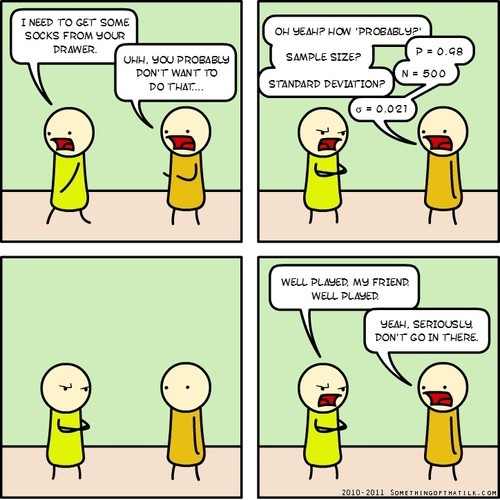
\includegraphics[height=.8\textheight]{img/intro-01.jpg}
\end{frame}

\begin{frame}
  \frametitle{Doel van deze cursus}
  
  \begin{itemize}
    \item Inleiding data science/statistiek
    \item Voorbereiding bachelorproef
  \end{itemize}
\end{frame}

\begin{frame}
  \frametitle{Hoe het niet moet}
  
  \centering
  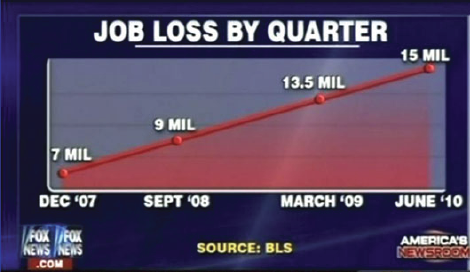
\includegraphics[height=.8\textheight]{img/intro-02.png}
\end{frame}

\begin{frame}
  \frametitle{Hoe het niet moet}
  
  \centering
  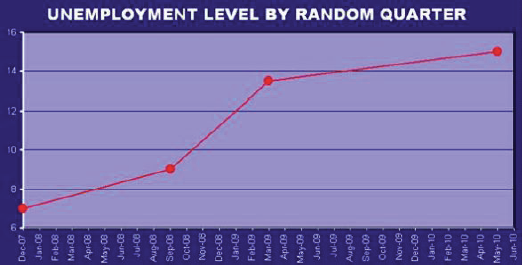
\includegraphics[height=.8\textheight]{img/intro-03.png}
\end{frame}

\begin{frame}
  \frametitle{Hoe het niet moet}

  \centering
  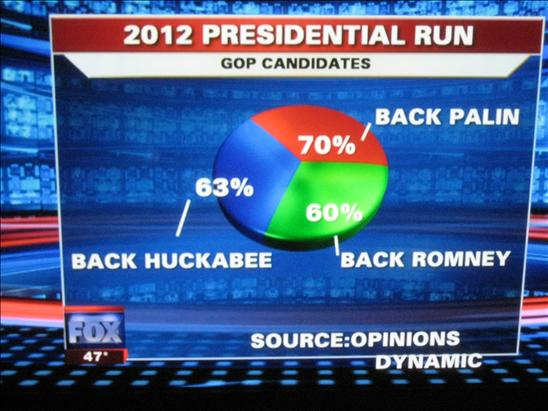
\includegraphics[height=.8\textheight]{img/intro-04.png}
\end{frame}

\begin{frame}
  \frametitle{Hoe het niet moet}

  \centering
  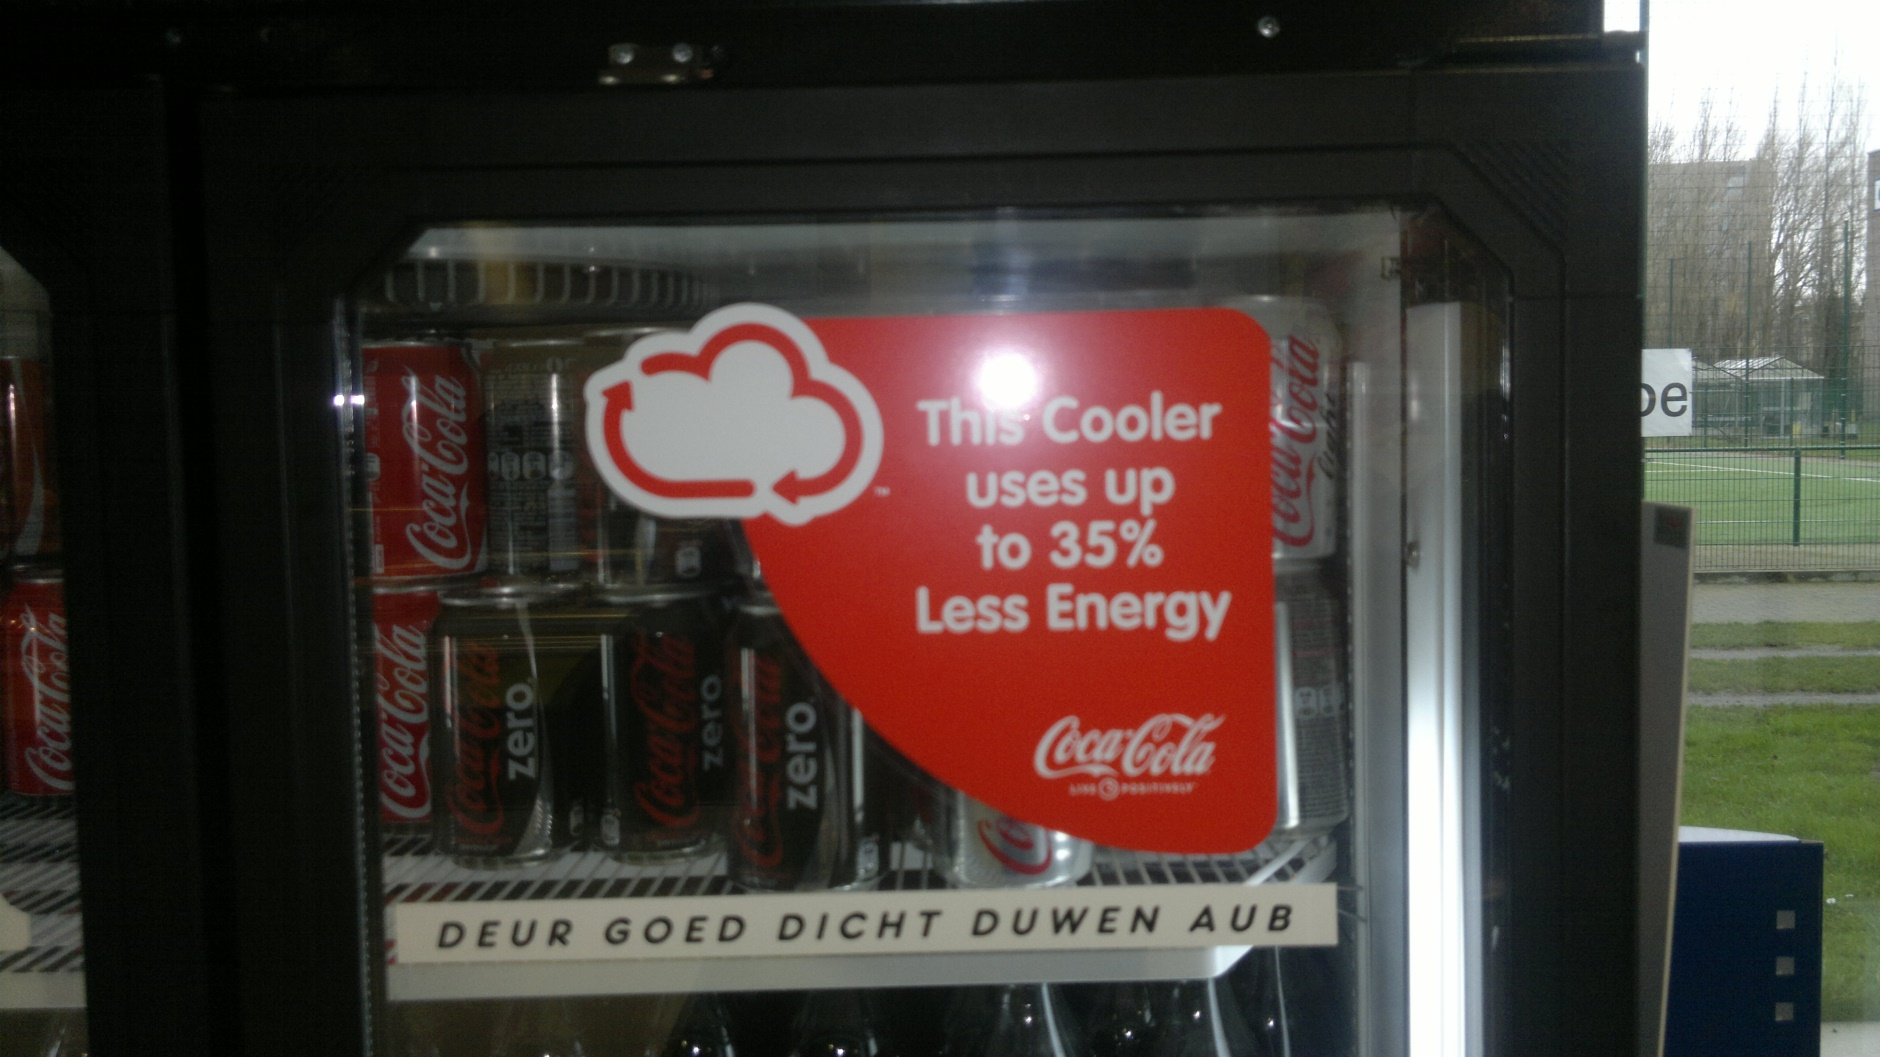
\includegraphics[height=.8\textheight]{img/intro-05.jpg}
\end{frame}

\begin{frame}
  \frametitle{Hoe het niet moet}

  \centering
  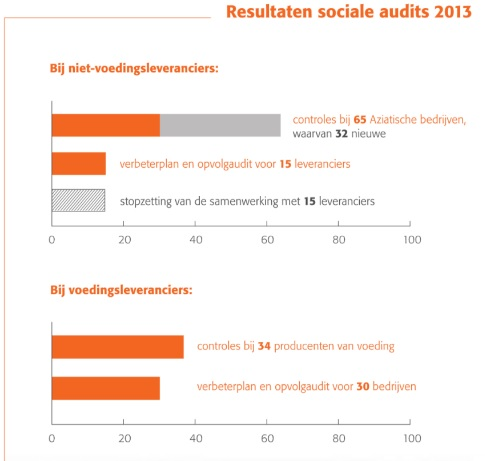
\includegraphics[height=.8\textheight]{img/intro-10.jpg}
\end{frame}

\begin{frame}
  \frametitle{Hoe het niet moet}
  {\tiny \textit{'Het overheidsbeslag is afgelopen jaar gedaald, maar niet zo spectaculair als een grafiek van de N-VA doet uitschijnen. Economieprofessor Tom Verbeke zag dat en wees N-VA met de vinger. 'Als een student dat soort truken toepast, zal hij zich serieus mogen verdedigen.'} }
  
  \centering
  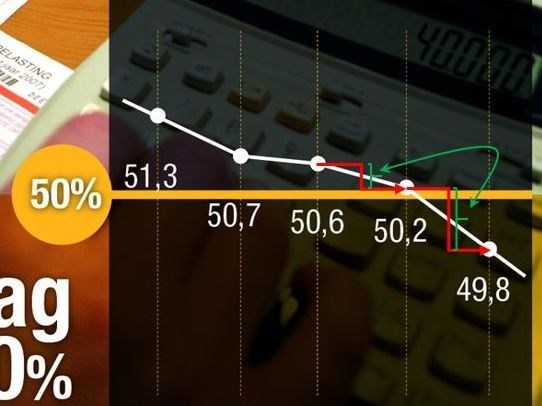
\includegraphics[height=.7\textheight]{img/intro-nva.jpg}
\end{frame}

\section{Praktisch}

\begin{frame}
  \frametitle{Overzicht leerstof}

\begin{table}[h]
\begin{tabular}{l|l}
  \multirow{2}{*}{\textbf{Inleiding}} &
     \tabitem Inleiding tot het vak \\
   & \tabitem Invoer van gegevens \\

  \hline
  \multirow{2}{*}{\textbf{Analyse op 1 variabele}} &
      \tabitem Enkelvoudige statistieken \\
    & \tabitem Eenvoudige grafieken\\

  \hline
  \multirow{2}{*}{\textbf{Analyse op 2 variabelen}} &
      \tabitem Eenvoudige grafieken \\
    & \tabitem Correlatie en regressie\\

  \hline
  \multirow{3}{*}{\textbf{Steekproeven en kansverdeling}} &
      \tabitem Populatie\\
    & \tabitem Steekproef\\
    & \tabitem Normale verdeling\\

\end{tabular}
\end{table}
\end{frame}
\begin{frame}
\frametitle{Overzicht leerstof (vervolg)}

\begin{table}[h]
  \begin{tabular}{l|l}

    \textbf{Toetsingsprocedure en} & \tabitem Toetsen van hypothesen \\
    \textbf{Chi-kwadraattoets}     & \tabitem $z$-toets, $t$-toets\\
    & \tabitem $\chi^{2}$-toets\\
    
    \hline
    \multirow{3}{*}{\textbf{Tijdreeksen}} &
    \tabitem Wiskundige modellen \\
    & \tabitem Voortschrijdend gemiddelde\\
    & \tabitem Exponentiële afvlakking\\
  \end{tabular}
\end{table}
\end{frame}

\begin{frame}
  \frametitle{Leermaterialen}

  \begin{itemize}
    \item Cursus (via Chamilo, Github)
    \item Slides ter ondersteuning
      \begin{itemize}
        \item bevatten grafieken en tabellen die in de les aan bod komen
      \end{itemize}
    \item Theorie aan bord, hoorcollege
      \begin{itemize}
        \item Volg de lessen \textbf{actief} mee!
        \item \textbf{Neem zelf notities!}
      \end{itemize}
  \end{itemize}

  \alertbox{Kom naar de les en \textcolor{hgyellow}{neem nota's}!}

  \begin{center}
    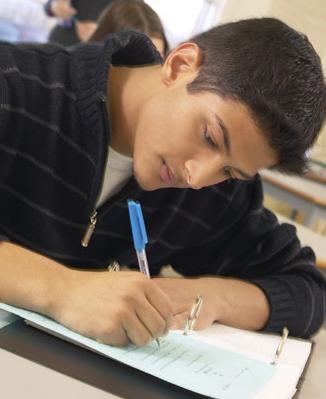
\includegraphics[height=3cm]{img/intro-06.jpg}
  \end{center}

\end{frame}

\begin{frame}
  \frametitle{Effectieve studiemethoden}
  
  Slagingspercentage in 1e zit: $\sim35\%$ (dag), $\sim10\%$ (TILE)
  
  \vspace{8pt}
  
  Gebruik effectieve studiemethoden:
  
  \begin{itemize}
    \item Retrieval practice
    \item Spaced practice
    \item Elaboration
    \item Interleaving
    \item Concrete voorbeelden
    \item Dual coding
  \end{itemize}

  Zie studiewijzer, \url{http://www.learningscientists.org/}
  
  \alertbox{Werk tijdens het semester!}
\end{frame}

\begin{frame}
  \frametitle{Software}
  
  Instructies: zie cursus, hst 1.
  
  \begin{itemize}
      \item Git:
      \begin{itemize}
          \item Git client
          \item Account op Github
      \end{itemize}
      \item {\LaTeX}:
      \begin{itemize}
          \item MikTeX/MacTeX/Texlive
          \item TexStudio (of andere editor)
          \item JabRef (bibliografische databank)
      \end{itemize}
      \item Statistiek: R, RStudio Desktop
  \end{itemize}

  \centering
  Alle benodigde software is gratis/open source
\end{frame}

\begin{frame}
  \frametitle{Organisatie van de lessen}

  \begin{itemize}
    \item Hoorcollege
      \begin{itemize}
        \item Theorie en grondleggen van de basis
      \end{itemize}
    \item Werkcollege
      \begin{itemize}
        \item Uitdiepen van de kennis
        \item Klassikaal oefeningen maken
        \item De software leren gebruiken
      \end{itemize}
    \item Begeleide zelfstudie
      \begin{itemize}
        \item Klassikaal taak uitwerken
        \item ``Passieve'' begeleiding
      \end{itemize}
  \end{itemize}
\end{frame}

\begin{frame}
  \frametitle{Evaluatie van het vak}

  \begin{itemize}
    \item Eerste examenkans
      \begin{itemize}
        \item Niet-periodegebonden evaluatie (taak): 30\% van het totaal
          \begin{itemize}
            \item Empirisch onderzoek in groep
          \end{itemize}
        \item Periodegebonden evaluatie (examen): 70\% van het totaal
        \begin{itemize}
          \item Schriftelijk gesloten boek (theorie)
          \item Schriftelijk met voorbereiding op eigen laptop (oefeningen)
        \end{itemize}
      \end{itemize}
    \item Tweede examenkans
      \begin{itemize}
        \item Niet-periodegebonden evaluatie: 30\%, \textbf{overgenomen uit 1e zit}
        \item Periodegebonden evaluatie: 70\% (idem 1e zit)
      \end{itemize}
  \end{itemize}

  \begin{center}
    
\includegraphics[height=3cm]{img/intro-07}
  \end{center}
\end{frame}

\begin{frame}
  \frametitle{NPE: Casus onderzoeksproces}

  \alertbox{Kunnen goede studietechnieken invloed hebben op resultaat?}

  \begin{enumerate}
    \item Literatuuronderzoek
    \item Experimenten reproduceren
    \item Onderzoeksvraag bijsturen, afbakenen en vastleggen
    \item Uitvoeren van de tests op een gecontroleerde manier.
    \item Resultaten statistisch verantwoord verklaren en neerschrijven
    \item Verslaggeving over het onderzoek
  \end{enumerate}

  Opdrachtbeschrijving op Chamilo, onder Opdrachten
\end{frame}

%---------- Back matter -------------------------------------------------------

\end{document}
